\documentclass{standalone}
\usepackage{pgfplots}
\usetikzlibrary{shapes.geometric, intersections, calc}
\pgfplotsset{compat=1.7}

\begin{document}
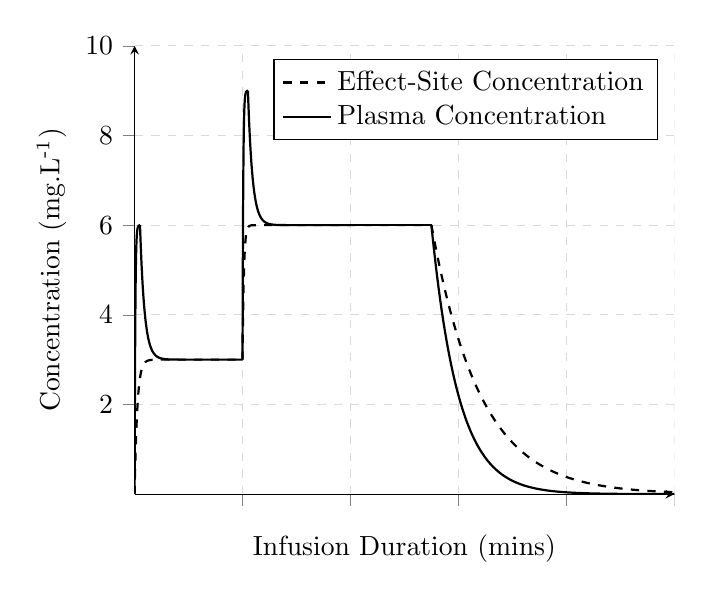
\begin{tikzpicture}

    \begin{axis}[
        axis x line=middle,
        axis y line=middle,
        grid = major,
        grid style={dashed, gray!30},
        xmin=0,     % start the diagram at this x-coordinate
        xmax= 10,    % end   the diagram at this x-coordinate
        ymin= 0,     % start the diagram at this y-coordinate
        ymax= 10,   % end   the diagram at this y-coordinate
        %axis background/.style={fill=white},
    	  x label style={at={(axis description cs:0.5,-0.1)},anchor=north},
	  y label style={at={(axis description cs:-0.1,.5)},rotate=90,anchor=south},
	  xticklabels={},
	 yticklabels={2,4,2,4,6,8,10},
	xlabel near ticks,
ylabel near ticks,
        xlabel=Infusion Duration (mins),
        ylabel=Concentration (mg.L\textsuperscript{-1}),
        tick align=outside,
        enlargelimits=false,
legend pos=north east,
legend cell align={left}]

	\addplot[domain=0:2, black, dashed, thick,samples=500] {3*(1-exp(-20*x))};
	\addplot[domain=0:0.10, black, thick,samples=500] {6*(1-exp(-80*x))};
	\addplot[domain=0.1:2, black, thick,samples=500] {3*exp(-12*(x-0.1))+3};
	\addplot[domain=2:2.10, black, thick,samples=500] {6*(1-exp(-80*(x-2)))+3};
	\addplot[domain=2.1:4, black, thick,samples=500] {3*exp(-12*(x-2.1))+6};
	\addplot[domain=4:5.5,black,thick,samples=500] {6};
	\addplot[domain=5.5:10, black, thick,samples=500] {6*exp(-2*(x-5.5))};
	\addplot[domain=2:5.5, black, dashed, thick,samples=500] {3*(1-exp(-2*(20*(x-2))))+3};
	\addplot[domain=5.5:10, black, dashed, thick,samples=500] {6*exp(-1.1*(x-5.5))};

	\addlegendentry{Effect-Site Concentration}
	\addlegendentry{Plasma Concentration}

\end{axis}

\end{tikzpicture} 
\end{document}